\section{GNSS Principles}
\label{gnss_principles}

In this section, we will talk about
a particular type of sensor  the Global Navigation Satellite
Systems or GNSS receiver. We will learn about why
this navigation sensor is so important for a self-driving car. It is able to provide a
position fix anywhere in the world with bounded
error which is a key. 

Specifically, we will develop a model for GNSS based on the principles of
pseudoranging and trilateration. We will then familiarize ourselves
with sources of GNSS positioning error and talk about some ways
to improve one type of GNSS. 



Just like the IMU discussed in a previous lecture, nearly every modern smartphone has
at least one type of GNSS receiver. Although we take them for granted now, the first modern system of
global positioning satellites, GPS, was built for military use during the 1980s. 
By the time the second version of the system was fully operational in 1995, GPS was made available
to the public for free. This was in part due to
the highly publicized crash of Korean Airlines flight 007 in 1983. Flight 007 was a 747
passenger jet that flew from New York City to Seoul with
refueling stop in Anchorage Alaska. As it flew from Anchorage to Seoul, it deviated from its plan flight path
and was shot down by a fighter jet after spending
several hours in Soviet airspace. To cross the North Pacific Ocean, Flight 007 relied on an inertial
navigation system for guidance. The pilots, failing to properly
initialize the system, mistakenly maintained the aircraft
on a specific magnetic heading. In turn, the plane deviated by more than 300 kilometers
from its planned course. Shortly after Flight 007 was shot down, then President Ronald Reagan
issued a directive to allow the US Global Positioning System to be freely available to the public
once it was fully developed. Although GPS was the original system of navigation satellites used for
global positioning, today, the term global navigation
satellite system is used as a catch-all for several such satellite
constellations that exist. The two that are fully
operational as of 2018 are GPS and GLONASS, the Russian equivalent. Several other systems
are nearing completion including the European
Galileo constellation. 


\subsection{The GPS system} 

Although, we will focus on the GPS, other GNSS systems
operate on similar principles. 


The GPS constellation is composed of 24-32 satellites that are
in six orbital planes. Satellites are decommissioned
and replaced periodically. Each satellite is at a medium Earth
orbit an altitude of roughly 20,000 kilometers with an orbital period
of just under 12 hours. The constellation is designed such
that at least four satellites are visible at any surface point
on earth at all times. Each satellite broadcasts
on two frequencies, one for civilian and
one for military use. Each broadcast signal contains
a pseudo-random code that identifies the satellite position and the time of transmission of the signal. 

The basic principle behind GPS is time of arrival ranging. The receiver computes a distance
to each visible satellite by comparing its own internal clock with
that of the time of transmission. The time difference is converted
to a distance using knowledge that electromagnetic signals
propagate at the speed of light. In order to compute a 3D position, the ranging equations require
at least four visible satellites. If altitude is known and
only a 2D position is required, only three satellites are needed. The process of recovering position
from several distances to known landmarks is called trilateration. 


\begin{framed}
\theoremstyle{remark}
\begin{remark}{}

Note that this is different
from triangulation where we compute positions based
off of angle measurements. 
\end{remark}
\end{framed}


A GPS receiver measures the pseudorange
to each satellite using the following measurement model: 

\begin{equation}
\rho^{(i)} =  c (t_r - t_s) = \sqrt{(\mathbf{p}^{(i)} - \mathbf{r})^T(\mathbf{p}^{(i)} - \mathbf{r})} + c \Delta t_r + c\Delta t_{\alpha}^{(i)} + \eta^{(i)}
\end{equation}

where $\mathbf{r}$ is the receiver 3D position, $\mathbf{p}^{(i)}$ is the position of the $i-$the satelite, $\Delta t_r$ is the receiver clock error, 
$\Delta t_{\alpha}^{(i)}$ is the atmospheric propagation delay, $\eta$ is the measurement noise, $c$ is the speed of light and $t_s, t_r$ are the time sent and time received respectively.


The model accounts for receiver clock error, atmospheric propagation delays,
and measurement noise. The term pseudorange
refers to the fact that the range information is corrupted
by the error sources above. Each pseudorange measurement defines
a circle in 2D, see Figure \ref{gnss_1}, or a sphere in 3D. 


\begin{figure}[!htb]
\begin{center}
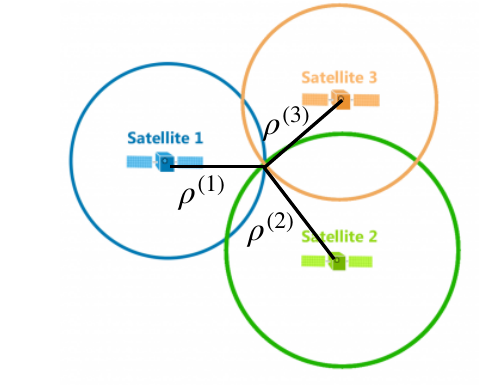
\includegraphics[scale=0.280]{img/hardware/gnss_1.jpeg}
\end{center}
\caption{Trilateration in 2D.}
\label{gnss_1}
\end{figure}


If we have exactly four satellites, we can solve for
the receiver position, $\mathbf{r}$, and the receiver clock error, $\Delta t_r$,  explicitly. If we have more than four, we can use the method of
least squares to find the maximum likelihood position
assuming Gaussian noise. GPS suffers from multiple error sources. First, charged ions in the ionosphere can delay
the signal by an unknown amount. Surrounding terrain and buildings
may cause reflections that increase the distance traveled by
the signal before reaching the receiver, these are called multi-path errors. Any small error in
clock synchronization or satellite position information can
have catastrophic consequences. Even a one microsecond
timing error can lead to a significant error in
position, 300 meters. Both a Ephemeris data
and satellite clocks are updated and recalibrated often, but the calibration can be out of date. Finally, the geometric configuration of visible satellites can also lead to
variations in positioning accuracy. This is known as the geometric
dilution of precision. For higher accuracy, a configuration with satellites spread across
the sky is preferable. 

Luckily, for some applications, we can improve GNSS accuracy by
augmenting the system in various ways. Differential GPS can correct receiver positioning
estimates by making use of the more accurately known positions
of one or more fixed base stations. Corrections are broadcast
on separate frequencies to the GNSS receiver in the moving vehicle. Real-Time Kinematic, or
RTK GPS makes use of carrier phase information to improve positioning accuracy down to
two centimeters in some cases. Although both of these techniques can significantly improve
the accuracy of GPS, they are typically quite
costly to implement. Inertial sensors are very
useful for navigation. However, they drift or accumulate
unbounded error over time. The GPS system in contrast, provides bounded error
positioning updates. A self-driving car equipped
with GPS will maintain a guaranteed level of positioning
accuracy at all times, unless the GPS receiver fails or loses
track of at least four satellites. 

\subsection{Summary}

To summarize, the Global Navigation Satellite
Systems work by combining pseudoranges from at least four
satellites to determine a 3D position. GPS or GNSS error can come from several different sources
including ionospheric delays, multi-path effects, and also possibly from the geometric
dilution of precision. In order to improve GNSS accuracy, techniques like differential GPS
or RTK GPS can be used.  We can fuse inertial
measurements from IMUs with position measurements
from a GPS to produce an accurate localization estimate
for a self-driving car. The sensors are complementary
and they're used together in practically all self-driving cars.

\subsection{Questions}

\subsection{Assignements}
 





